\documentclass[tikz,border=10pt]{standalone}
\begin{document}
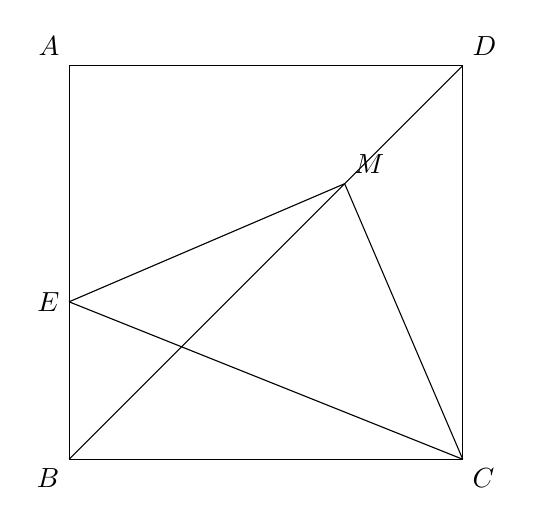
\begin{tikzpicture}
    \coordinate (A) at (0,5);
    \coordinate (B) at (0,0);
    \coordinate (C) at (5,0);
    \coordinate (D) at (5,5);
    \coordinate (E) at (0,2);
    \coordinate (M) at (3.5,3.5);

    \draw (A) -- (B) -- (C) -- (D) -- cycle;
    \draw (B) -- (D);
    \draw (E) -- (C);
    \draw (E) -- (M);
    \draw (M) -- (C);

    \node[above left] at (A) {$A$};
    \node[below left] at (B) {$B$};
    \node[below right] at (C) {$C$};
    \node[above right] at (D) {$D$};
    \node[left] at (E) {$E$};
    \node[above right] at (M) {$M$};
\end{tikzpicture}
\end{document}
